\documentclass{article}
% --- watermark (auto-inserted) ---
\usepackage{xcolor}
\usepackage{xfp}% \fpeval; in the kernel since 2022, harmless on older LaTeX
\usepackage{draftwatermark}
\newlength{\watermarkTextWidth}
\AddToHook{begindocument/end}{%
  \SetWatermarkText{\normalfont Generated by The Agentic Scientist}%
  \SetWatermarkFontSize{10pt}%
  \SetWatermarkLightness{0.85}%
  \settowidth{\watermarkTextWidth}{\normalfont\fontsize{10pt}{12pt}\selectfont Generated by The Agentic Scientist}%
  \edef\watermarkScale{\fpeval{0.8 * sqrt(\paperwidth**2 + \paperheight**2) / \watermarkTextWidth}}%
  \edef\watermarkAngle{\fpeval{atand(\paperheight/\paperwidth)}}%
  \SetWatermarkScale{\watermarkScale}%
  \SetWatermarkAngle{\watermarkAngle}%
}
% --- end watermark ---

\usepackage{paper,times}
\usepackage[T1]{fontenc}
\usepackage[utf8]{inputenc}
\usepackage{amsmath,amssymb,booktabs,graphicx,subcaption,xcolor}
\usepackage{hyperref,url}
\title{Missingness-Aware Latent Models for Budgeted\ Embedding Benchmark Prediction}
\author{}
\newcommand{\latent}{\textsc{Latent}}
\newcommand{\ridge}{\textsc{Ridge}}
\newcommand{\randomlr}{\textsc{Random-LR}}
\begin{document}
\maketitle

\begin{abstract}
Historical benchmark tables offer a way to predict a new model's performance without evaluating every benchmark, but incomplete coverage and model relatedness complicate this promise. We study sequential benchmark acquisition on naturally incomplete English MTEB embedding-model score panels. A historical-only procedure fits an observed-data factor model, considers a constrained latent-mixture extension, and selects benchmarks using conditional cross-task transfer. Evaluation separates model-group and name-proxy-family-disjoint holdouts and reserves never-queryable audit targets. Across the frozen split realizations and query budgets, remaining-target mean absolute error is 0.03130, compared with 0.03607 for greedy correlation coverage with ridge prediction and 0.04563 for random acquisition with low-rank prediction. The corresponding common-target audit errors are 0.02687, 0.02941, and 0.03547. One family-disjoint split reverses the comparison with ridge on both targets. Permuting historical columns substantially increases error. These descriptive results support the evaluated procedure within the recorded embedding panels, not universal benchmark sufficiency, component-specific gains, or generalization to generative language models.
% @evidence[[paper_data.json#/final_evaluation/metrics]]
% @evidence[[derived_results.json#/aggregate_original]]
% @evidence[[derived_results.json#/cases]]
\end{abstract}

\section{Introduction}
Broad language-model evaluation is multidimensional: knowledge and scenario-based evaluations measure different aspects of performance \citep{Hendrycks2021MMLU,Liang2023HELM}. Text embeddings likewise serve distinct applications, including classification, retrieval, clustering, and semantic similarity. MTEB makes this diversity explicit \citep{Muennighoff2023MTEB}. Evaluating each new embedding model on every benchmark can be burdensome. An alternative is to reuse the historical score table: evaluate a small panel for the new model, then infer its scores on the remaining benchmarks. The scientific question is not whether benchmarks are correlated in aggregate, but whether those relationships permit accurate prediction for held-out models under a specified acquisition budget.

Several obstacles make this a prediction problem rather than a leaderboard summarization problem. Historical entries are naturally missing; absence need not be independent of model capability or evaluation choices. A high score on one task need not imply comparable scores elsewhere. Related models can make randomly held-out rows deceptively easy. Moreover, an acquisition policy determines not only which values become available but which targets remain to be scored. A method can obtain a favorable remaining-target error partly by removing difficult targets through querying. A common, never-queryable target set is therefore necessary for interpreting the comparison.

We investigate a missingness-aware latent-model procedure on frozen English MTEB score panels. Its design combines observed-data factor analysis, an optional mixture over latent profiles, conditional prediction, and transfer-oriented acquisition. Historical row-held-out validation chooses among these configurations before the outer models are queried. This is a concrete integration of established statistical tools rather than a claim of a new latent-variable architecture. The hypothesis is that modeling shared variation and benchmark-specific residuals can provide a useful conditional predictor, while accommodating heterogeneous latent profiles may help when observed scores identify specialization. The latter mechanism remains a hypothesis unless isolated by controlled evidence.

The contribution is a bounded empirical characterization with three elements. First, we specify a historical-only predictor and acquisition rule that can operate on an incomplete score matrix. Second, we compare the frozen procedure with executed random-low-rank and greedy-coverage ridge pipelines under both model-group and name-proxy-family-disjoint holdouts. Third, we make unchanged audit targets, split variation, an adverse comparison, and destroyed historical alignment central to interpretation. The measured aggregate favors the latent procedure on both target definitions, but not uniformly across splits. No additional dataset, generative-model evaluation, or independently verified lineage annotation is available. The study thus addresses when the evaluated integration is useful in this retrospective setting, not how many benchmarks are universally sufficient.
% @evidence[[paper_data.json#/final_evaluation/evaluation_evidence/episodes]]

\begin{figure}[t]
\centering

\includegraphics[width=\linewidth]{figures/problem_and_evidence_overview.png}
\caption{Budgeted prediction and its evidence boundary. A masked historical score matrix supports fitting and internal model choice. Revealed benchmark scores condition predictions and may influence further acquisition. Outer audit columns are never queryable; only recorded target cells are scored. The common-target boundary separates predictive transfer from changes in which targets remain.}
\label{fig:overview}
% @evidence[[source_evidence/latent/program.py#handle]]
% @evidence[[source_evidence/protocol/evaluate_final.py#losses]]
\end{figure}

\section{Related Work}
\paragraph{Reducing evaluation and predicting performance.}
Item-level compression and whole-benchmark acquisition address different units of cost. \citet{Polo2024Tiny} study estimating benchmark performance from fewer examples; \citet{Kipnis2024Meta} construct a sparse assessment from informative items across reasoning and knowledge benchmarks. Here a query reveals one entire benchmark-context score, not an individual test response. Observational scaling laws exploit existing model evaluations instead of training new models \citep{Ruan2024Scaling}; skills-based scaling laws also study multi-benchmark prediction across model families \citep{Polo2024Sloth}. Our predictor receives historical score matrices and sequentially revealed scores, without training-compute covariates. These works motivate related questions, but they are not implemented comparison methods in this study. Their generative-model settings must not be conflated with the embedding panels measured here.

\paragraph{Incomplete matrices and latent profiles.}
Matrix factorization is a standard approach to sparse observations \citep{Koren2009Factors}. Convex matrix completion, noisy recovery, and few-entry recovery provide complementary formulations \citep{Candes2009Completion,Candes2010Noisy,Keshavan2010Completion}; spectral regularization offers another computational approach \citep{Mazumder2010Spectral}. Their recovery conditions do not automatically hold for selectively reported benchmark tables. Missing-data inference requires assumptions about the observation process \citep{Rubin1976Missing}. Our observed-data fitting uses EM-style latent sufficient statistics \citep{Dempster1977EM}, with a benchmark-specific diagonal residual rather than the isotropic residual of probabilistic PCA \citep{Tipping1999PPCA}.

Mixtures of factor analyzers supply a classical framework for combining latent factors and heterogeneous profiles \citep{Ghahramani1996Mixture}. Related formulations study factor-mixture dimensional reduction, cluster-weighted factors, efficient conditional maximization, deeper mixtures, and incomplete high-dimensional data \citep{Viroli2010Mixture,Subedi2012Mixture,Zhao2008ECM,Viroli2017Deep,Wei2017Missing}. The implemented extension here is narrower: shared loadings and diagonal residuals are frozen before fitting a small mixture over latent means. We neither reproduce those broader models nor establish their relative accuracy.

\paragraph{Acquisition and absolute-loss decisions.}
Bayesian experimental design and statistical active learning connect acquisition to posterior uncertainty and prediction objectives \citep{Chaloner1995Design,Cohn1996Active}. Absolute loss calls for a median rather than a mean under the predictive distribution; quantile regression and forecast assessment emphasize matching the action to the loss \citep{Koenker2001Quantiles,Gneiting2011Forecasts}. This motivates bounded posterior medians and a square-root-variance transfer heuristic. Loss alignment at prediction time does not make the acquisition heuristic an exact expected-risk optimizer, especially under a mixture posterior. Our contribution is the measured integration and its limits, not novelty of these statistical principles.

\section{Method}
\subsection{Problem Setup and Evaluation Target}
Let $X\in[0,1]^{M\times N}$ contain historical scores and let $R$ be their binary observation mask. A row denotes an embedding model; a column denotes a benchmark together with language, evaluation split, primary metric, and dataset revision. An unrecorded cell is missing, not a zero score. For a held-out model with score vector $y$, the evaluator exposes an available query set $A$. The policy selects distinct indices $S_k\subseteq A$ and observes $y_{S_k}$ under a budget $k$. Its prediction $\widehat y^{(k)}$ is evaluated only where a target score is recorded.

Write $O$ for the recorded target columns and $H$ for the audit columns, with $A=O\setminus H$. The two losses are
\begin{equation}
 L_{\rm rem}^{(k)}=\frac{\sum_{j\in O\setminus S_k}|\widehat y_j^{(k)}-y_j|}{|O\setminus S_k|},
 \qquad
 L_{\rm audit}^{(k)}=\frac{\sum_{j\in O\cap H}|\widehat y_j^{(k)}-y_j|}{|O\cap H|}.
 \label{eq:losses}
\end{equation}
% @evidence[[source_evidence/protocol/evaluate_final.py#losses]]
Remaining-target loss measures the practical residual prediction task but has method-dependent targets. Audit loss holds the scored cells fixed across methods and budgets within each held-out row. Both losses are needed: the former describes the acquisition-dependent task, while the latter tests prediction without removing difficult audit targets. Neither evaluates cells that were never measured in the public table.

\subsection{Design Rationale and Observed-Data Fitting}
The central design hypothesis is that shared cross-benchmark variation can be estimated without treating absent measurements as observed outcomes. We fit a Gaussian factor model
\begin{equation}
 x=b+Wz+\epsilon,\qquad z\sim\mathcal N(0,I),\quad
 \epsilon\sim\mathcal N(0,D),\quad \Sigma=WW^\top+D,
 \label{eq:factor}
\end{equation}
where $D$ is diagonal. Its entries represent benchmark-specific variation across models, not repeated-measurement noise. Historical means and scales are computed from recorded training entries. A zero-filled standardized matrix initializes the loadings by SVD, but subsequent likelihood contributions and sufficient statistics use only observed coordinates. This distinction matters: initialization does not turn zeros in missing cells into training labels.

For historical row $i$ with observed coordinates $O_i$, the latent posterior has covariance and mean
\begin{equation}
 V_i=(I+W_{O_i}^{\top}D_{O_i}^{-1}W_{O_i})^{-1},\qquad
 m_i=V_iW_{O_i}^{\top}D_{O_i}^{-1}(x_{i,O_i}-b_{O_i}).
 \label{eq:posterior}
\end{equation}
The loading and residual updates integrate $\mathbb E[zz^\top\mid x_{i,O_i}]=V_i+m_im_i^\top$. Each benchmark's update uses rows where that benchmark is recorded. Diagonal regularization stabilizes the linear solves; shrinkage and a variance floor prevent nearly singular residuals. This models the observed score distribution without supplying a model for why particular leaderboard entries are missing.
% @evidence[[source_evidence/latent/covariance.py#ResidualCovariance.fit]]

\subsection{Conditional Prediction and Heterogeneous Profiles}
A single Gaussian gives a clipped conditional mean,
\begin{equation}
 \widehat y=\operatorname{clip}_{[0,1]}
 \left[b+\Sigma_{:,S}(\Sigma_{S,S}+\delta I)^{-1}(y_S-b_S)\right],
 \label{eq:gaussian}
\end{equation}
with queried coordinates restored to their observed values. For this symmetric conditional distribution, the clipped mean is also a constrained median. The mixture extension retains $b,W,D$ and replaces the latent prior by
\begin{equation}
 p(z)=\sum_{g=1}^{G}\pi_g\mathcal N(z;a_g,\tau^2I),\qquad
 \mu_g=b+Wa_g,\qquad C=\tau^2WW^\top+D.
 \label{eq:mixture}
\end{equation}
The single-component alternative is the original Gaussian, not a separately fitted approximation. For multiple components, observed-data EM fits the masses, latent centers, and shared latent variance with regularization. Each revealed score updates component probabilities, conditional means, and their shared within-component covariance. Distinct target rows receive independent conditional states.

For each unqueried benchmark the mixture predictor approximately solves
$\sum_g\pi_g\Phi((a-\mu_{g,j})/\sqrt{C_{jj}})=1/2$ on $a\in[0,1]$ by bisection, choosing a boundary if the unconstrained median is outside the interval. This is the constrained Bayes action for modeled absolute error: where differentiable, the derivative of $\mathbb E|Y-a|$ is $2F_Y(a)-1$. The argument concerns the fitted predictive distribution, not the true distribution of new embedding models. It supplies no real-data optimality or uncertainty-calibration guarantee.
% @evidence[[source_evidence/latent/mixture.py#LatentMixture.fit_profiles]]
% @evidence[[source_evidence/latent/mixture.py#MixtureRow.reveal]]
% @evidence[[source_evidence/latent/mixture.py#MixtureRow.predict]]

\subsection{Transfer-Oriented Acquisition}
Let $T$ be the current modeled covariance, including between-component variation when a mixture is used. For candidate $q\in A\setminus S$, the variance-transfer score is
\begin{equation}
 U_{\rm var}(q)=\sum_{j\notin S\cup\{q\}}\frac{T_{jq}^2}{\max(T_{qq},\delta)}.
 \label{eq:transfer}
\end{equation}
For a Gaussian, this sums the conditional variance reductions on other columns. Excluding $q$ prevents a benchmark from receiving credit merely for revealing its own score. All modeled unobserved columns enter this utility, including columns unavailable for querying; the policy is not given the outer audit labels. Consequently its utility is not identical to either scored loss in Equation~\ref{eq:losses}.

A second selectable criterion replaces variance reduction with the sum of square-root reductions,
\begin{equation}
 U_{\rm sqrt}(q)=\sum_{j\notin S\cup\{q\}}
 \left[\sqrt{T_{jj}}-
 \sqrt{\max\{T_{jj}-T_{jq}^2/\max(T_{qq},\delta),0\}}\right].
 \label{eq:sqrt}
\end{equation}
The motivation is the relation between Gaussian absolute risk and standard deviation. Under a mixture, the total covariance is moment matched and depends on revealed values through posterior component weights. Equation~\ref{eq:sqrt} is nevertheless a heuristic: it does not integrate over possible queried values or recompute the expected bounded-mixture median risk. A single Gaussian's acquisition is score-value independent, although its predictions are not. We do not infer that value-dependent acquisition was used in every evaluated fit.
% @evidence[[source_evidence/latent/covariance.py#transfer_select]]
% @evidence[[source_evidence/latent/mixture.py#MixtureRow.select]]

\subsection{Historical Model Choice and Compared Pipelines}
The complete procedure, denoted \latent, chooses rank and residual shrinkage using a historical row split with fixed internal audit columns. It compares the Gaussian with a small set of mixture sizes, regularization strengths, and the two acquisition criteria. A configuration replaces the Gaussian only if its internal audit error improves beyond a margin based on paired historical-row differences. It is refitted on all supplied historical rows; insufficient validation or numerical failure falls back to the Gaussian. These are executable safeguards, not externally measured component ablations. The outer evidence does not establish which component counts, selectors, or fallbacks were realized, and internally reported diagnostics are not independently verified.

\randomlr\ uses random acquisition and a masked alternating-ridge low-rank predictor, with historical cell-held-out tuning. \ridge\ greedily covers squared historical correlations, shrunk according to pairwise overlap, and predicts each target by ridge regression on the selected scores. Its masked, centered historical predictors are zero at missing coordinates. The historical-mean reference predicts each benchmark's recorded training mean. Unlike matched acquisition ablations, these comparisons vary both acquisition and prediction. Any measured advantage belongs to the complete evaluated configuration, not solely to residual modeling, mixtures, medians, or the acquisition criterion. Supplementary Information gives source locations and numerical settings.
% @evidence[[source_evidence/latent/mixture.py#tune_fit]]
% @evidence[[source_evidence/protocol/evaluate_final.py#native_random]]
% @evidence[[source_evidence/protocol/evaluate_final.py#native_ridge]]

\section{Experimental Setup}
\paragraph{Data and scope.}
The frozen source is the public MTEB results repository at revision \texttt{6dabbcc68c28ea5f180ce7df79347b3ca9cc6383}. Each evaluation panel contains 48 benchmark-context columns and 48 held-out rows, with natural missingness retained. Classification accuracy, clustering V-measure, retrieval NDCG, and reranking MAP are treated on their declared unit intervals; signed Spearman correlations are mapped by $(s+1)/2$. Dataset revisions remain part of column identity. No imputed cell is a target, and no held-out extrema determine normalization. Historical coverage determines panel membership. Held-out row inclusion depends on recorded availability, not observed error. This is an embedding-model study on English panels, not an evaluation of generative language models or all tasks in the upstream repository.
% @evidence[[paper_data.json#/final_evaluation/evaluation_evidence/episodes]]
% @evidence[[source_evidence/protocol/data_manifest.json]]
% @evidence[[source_evidence/protocol/evaluate_final.py#score_cells]]

\paragraph{Holdouts and controls.}
Model-group holdouts separate identity components defined using normalized source content. The stricter condition additionally separates name-defined family proxies between historical and held-out rows. These proxies are not independently verified model genealogies. Frozen development and final pools are separated using normalized document and complete-row content checks; within each final split, the evaluator rechecks component and document disjointness. This reduces a specific form of duplication, not every possible form of evaluation contamination.

The final split seeds are 4001, 4009, and 4021. Query checkpoints are $k\in\{1,2,4,8\}$, and eight columns are never queryable audit columns. Only recorded audit cells are scored; not every held-out row has all audit measurements. Query availability is its recorded mask minus these columns, an explicitly retrospective constraint. A column-wise permutation control shuffles scores among recorded historical positions, preserving masks and each column's marginal values while disrupting cross-task alignment. Models and internal choices are refitted on the transformed history. A required deterministic reset replay is retained as a protocol diagnostic but receives no weight in accuracy summaries.
% @evidence[[paper_data.json#/final_evaluation/evaluation_evidence/episodes]]
% @evidence[[source_evidence/protocol/data_manifest.json#/production]]
% @evidence[[source_evidence/protocol/evaluate_final.py#permute_history]]

\paragraph{Aggregation and uncertainty.}
We average checkpoints equally within a row. Model-group summaries weight rows equally; family-disjoint summaries first average rows within a proxy family and then weight families equally. The final aggregate weights each original, non-replay condition--seed case equally. Historical-mean remaining-target errors use \latent's remaining sets; the common-audit mean does not depend on its selections. The final evaluation completed and met its operational qualification checks. This status is separate from predictive competitiveness and cannot replace scientific qualification of a broader claim.
% @evidence[[source_evidence/protocol/evaluate_final.py#row_average]]
% @evidence[[source_evidence/protocol/evaluate_final.py#plane_metrics]]
% @evidence[[paper_data.json#/grounding_sources/final.qualification.status/value]]
% @evidence[[paper_data.json#/grounding_sources/final.qualification.outcome/value]]

The seeds define frozen split realizations, not independent population draws or repeated fits to one identical test set. Rows and families can recur across splits. We therefore show raw split values and descriptive means, without row-level pseudo-replication, significance tests, or confidence intervals presented as independent-population uncertainty. Model selection used historical data only; the final measurements are reported separately from development scores. No additional evaluations were run for this manuscript.

\section{Results}
\subsection{Aggregate Accuracy on Remaining and Common Targets}
Table~\ref{tab:main} reports the frozen comparison. \latent\ has lower aggregate error than both executed predictive pipelines on the remaining-target objective. However, remaining sets differ between policies. The audit comparison is therefore essential: \latent's common-target error is also lower, showing that its aggregate advantage is not confined to the acquisition-dependent target definition. The absolute values are normalized score errors; a unit-normalized accuracy difference and a transformed correlation difference do not have identical application-level meanings.

\begin{table}[t]
\centering
\caption{Frozen aggregate normalized MAE; lower is better. Audit cells are never queryable. Means equally weight condition--seed cases after the prescribed row/family aggregation. These are descriptive comparisons, not significance claims.}
\label{tab:main}
\begin{tabular}{lrr}
\toprule
Pipeline & Remaining targets & Common audit targets \\
\midrule
\latent & 0.03130 & 0.02687 \\
\ridge & 0.03607 & 0.02941 \\
\randomlr & 0.04563 & 0.03547 \\
Historical mean & 0.08782 & 0.06056 \\
\bottomrule
\end{tabular}
% @evidence[[paper_data.json#/final_evaluation/metrics]]
% @evidence[[derived_results.json#/aggregate_original]]
\end{table}

The historical mean is substantially less accurate in aggregate on both target definitions, indicating that a benchmark-specific constant is insufficient for these evaluated panels. This does not establish the value of any particular component of \latent: conditional predictors with different fitting and selection choices also improve over the mean. Nor does the aggregate measure prediction of naturally unrecorded cells, for which no truth is available. The smaller audit errors should not be interpreted as intrinsically easier prediction by the same numerical factor: the fixed audit columns form a different, coverage-selected target set.

\subsection{Budget Trade-Offs on Unchanged Targets}
Figure~\ref{fig:budget} holds audit cells unchanged as the query budget increases. For model-group holdouts, \latent's descriptive mean audit MAE decreases from 0.03286 at one query to 0.01700 at eight; the corresponding \ridge\ values are 0.03411 and 0.02156. For family-disjoint holdouts, \latent\ decreases from 0.03880 to 0.02084, compared with 0.04084 to 0.02273 for \ridge. The family-disjoint mean at two queries favors \ridge\ (0.03153 versus 0.03363), so even the budget-specific ordering is not uniform. Additional observations help the descriptive mean within the measured range, but no predefined acceptable-error threshold or universal sufficient budget was tested.
% @evidence[[derived_results.json#/audit_budget_curves]]

\begin{figure}[t]
\centering
\begin{subfigure}{0.487\linewidth}
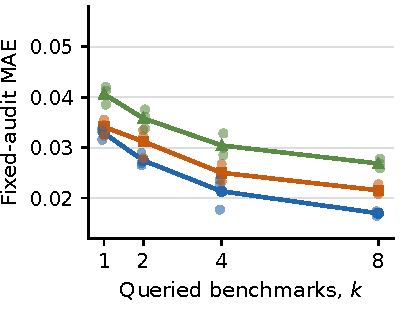
\includegraphics[width=\linewidth]{figures/common_target_budget_comparison_model_group.pdf}
\caption{Model-group holdout}
\end{subfigure}\hfill
\begin{subfigure}{0.487\linewidth}
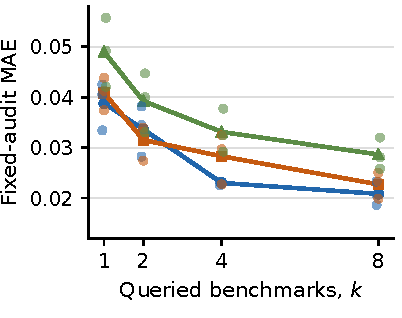
\includegraphics[width=\linewidth]{figures/common_target_budget_comparison_family_disjoint.pdf}
\caption{Name-proxy-family-disjoint holdout}
\end{subfigure}
\caption{Query-budget trade-offs on fixed audit targets. Blue circles: \latent; orange squares: \ridge; green triangles: \randomlr. Lines summarize descriptive means; small unconnected points show the individual split-seed values, not additional independent replications. Both panels share the same error scale.}
\label{fig:budget}
% @evidence[[derived_results.json#/audit_budget_curves]]
\end{figure}

The fixed-target design distinguishes information gain from target removal: the audit scores improve even though none of those columns can be acquired. Yet increasing the number of benchmark queries is not itself a measured saving in compute, wall-clock time, or money. Benchmarks have unequal costs and their scores may have different estimation uncertainty. The present objective weights normalized score errors rather than downstream decisions or evaluation cost. Choosing a deployment budget would require a desired accuracy, a cost model, and an evaluation distribution representative of future models, none of which is established by these curves.

\subsection{Split Variation and an Adverse Family-Disjoint Case}
Table~\ref{tab:splits} retains every original condition--seed comparison with the stronger baseline. The aggregate advantage is not uniform. For family-disjoint seed 4021, remaining-target MAE is 0.03666 for \latent\ and 0.03414 for \ridge; common-audit MAE is 0.02972 and 0.02687, respectively. Because the reversal also occurs on unchanged targets, it cannot be dismissed solely as a consequence of removing different queried columns. This is a measured performance reversal, not evidence identifying a validity failure, an adaptivity defect, or a particular family as its cause.
% @evidence[[derived_results.json#/cases]]

\begin{table}[t]
\centering
\caption{All original split summaries against ridge. Each entry already averages query checkpoints, with equal-row or equal-proxy-family weighting as appropriate. The adverse family-disjoint split remains visible on both losses.}
\label{tab:splits}
\begin{tabular}{llrrrr}
\toprule
& & \multicolumn{2}{c}{Remaining targets} & \multicolumn{2}{c}{Common audit targets} \\
Holdout & Seed & \latent & \ridge & \latent & \ridge \\
\midrule
Model-group & 4001 & 0.02814 & 0.03170 & 0.02571 & 0.02797 \\
Model-group & 4009 & 0.02975 & 0.03308 & 0.02480 & 0.02882 \\
Model-group & 4021 & 0.02714 & 0.03645 & 0.02349 & 0.02713 \\
Family-disjoint & 4001 & 0.03208 & 0.04392 & 0.02704 & 0.03186 \\
Family-disjoint & 4009 & 0.03402 & 0.03713 & 0.03047 & 0.03381 \\
Family-disjoint & 4021 & 0.03666 & 0.03414 & 0.02972 & 0.02687 \\
\bottomrule
\end{tabular}
% @evidence[[derived_results.json#/cases]]
\end{table}

The rows are split realizations, not disjoint experimental populations. They reveal heterogeneity that a single pooled error hides but do not supply a reliable population confidence interval. Equal-family weighting limits the influence of prolific proxy groups within a case; it does not correct misclassified lineage, all selection bias, or dependence across cases. Internal paired validation margins should not be confused with final paired uncertainty for these comparisons. Without externally verified matched ablations or family-cluster uncertainty, a mechanism-specific or statistically significant superiority claim would exceed the available evidence.

\subsection{Dependence on Historical Cross-Task Alignment}
Historical-column permutation changes \latent's remaining-target MAE from 0.03130 to 0.08976. Figure~\ref{fig:alignment} shows the corresponding common-target comparison for all predictive pipelines, separated by holdout condition. The increase also occurs on unchanged audit targets, consistent with these predictors exploiting useful historical cross-task alignment rather than only marginal benchmark means. This interpretation is deliberately descriptive. The transformation refits and retunes the entire pipeline, and can alter its selected configuration. It does not isolate covariance estimation, latent-mixture inference, or score-value adaptation.
% @evidence[[paper_data.json#/final_evaluation/metrics/candidate_mae]]
% @evidence[[paper_data.json#/final_evaluation/metrics/permuted_mae]]
% @evidence[[derived_results.json#/cases]]

\begin{figure}[t]
\centering
\begin{subfigure}{0.487\linewidth}
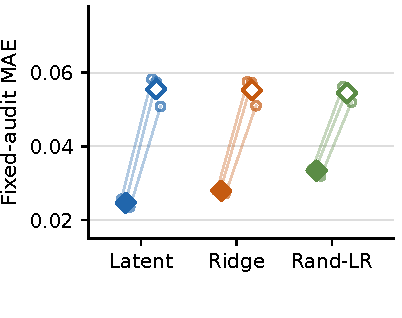
\includegraphics[width=\linewidth]{figures/historical_alignment_control_model_group.pdf}
\caption{Model-group holdout}
\end{subfigure}\hfill
\begin{subfigure}{0.487\linewidth}
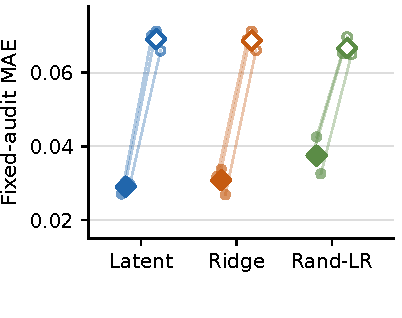
\includegraphics[width=\linewidth]{figures/historical_alignment_control_family_disjoint.pdf}
\caption{Name-proxy-family-disjoint holdout}
\end{subfigure}
\caption{Historical-alignment control on common audit targets. Filled markers use original history; open markers use column-permuted history. Small paired circles are split values; large diamonds are descriptive means across splits. Each value averages query checkpoints. Colors match Figure~\ref{fig:budget}. Permutation preserves column marginals and masks but changes joint structure and refits the complete predictor.}
\label{fig:alignment}
% @evidence[[derived_results.json#/cases]]
\end{figure}

The control cannot distinguish shared capability from correlated reporting, benchmark overlap, or other joint structure in the historical table. It also does not simulate a realistic future distribution shift. Its purpose is narrower: after destroying observed alignment while retaining column marginals and the missingness mask, the recorded predictive accuracy deteriorates. The deliberately weak queried-score-average reference and deterministic replay are reported separately in Supplementary Information rather than treated as competing explanations of the main comparison.

\section{Discussion and Limitations}
\paragraph{What the comparison establishes.}
The evidence supports lower aggregate error for the frozen \latent\ procedure than for the two executed predictive baselines on these recorded English embedding panels. The common-target comparison strengthens this finding because scored audit cells do not change with acquisition. It remains a comparison among evaluated complete configurations. In particular, the data do not establish that mixtures were selected, that a mixture outperformed a Gaussian under matched queries, or that the square-root criterion improved over variance transfer. Their static implementation is inspectable; their individual empirical contributions are not externally verified.

\paragraph{Missingness and target availability.}
Observed-data likelihood avoids fitting absent cells as zeros, but it does not make leaderboard missingness ignorable. Model inclusion, panel coverage, and the requirement of recorded audit scores restrict the evaluated population. The query interface assumes knowledge of which historical target entries exist; a prospective evaluator may instead be able to run different tasks or face uncertain availability. Naturally unrecorded scores remain unevaluated. Likewise, averaging normalized heterogeneous metrics is convenient for prediction error but need not match the evaluator's utility. No sensitivity study over alternative missingness mechanisms, target weights, or task-cost schedules is available.

\paragraph{Generalization and evidence strength.}
Name-derived families are proxies for lineage, and content disjointness addresses a narrower issue than architectural or training-data independence. The adverse family-disjoint split rules out a uniform advantage over the stronger baseline. Small, potentially overlapping split sets preclude strong population-level claims from the descriptive averages. A further benchmark source, multilingual coverage, larger acquisition budgets, calibrated predictive intervals, and a prospective new-model study are not measured. None should be inferred from operational qualification or the existence of a reproducible score extraction procedure. Predictions should complement direct measurement, not be relabeled as measured benchmark results.

\paragraph{Practical interpretation.}
The procedure is appropriate as a candidate tool when historical cross-task relationships are informative, comparable benchmark contexts can be identified, and the target resembles the represented population closely enough for conditional transfer. The observed degradation under permutation and heterogeneous split behavior provide reasons to monitor this assumption rather than assume it. A deployment should preserve a directly evaluated audit panel and expose prediction uncertainty and provenance. These are cautions motivated by the study, not capabilities validated for the present implementation.

\section{Conclusion}
Budgeted benchmark prediction requires evaluating both a selection policy and the predictor it enables. On naturally incomplete English MTEB panels, the studied missingness-aware latent procedure obtains lower aggregate normalized absolute error than random-acquisition low-rank and greedy-coverage ridge pipelines. Its advantage persists on never-queryable audit targets, but a family-disjoint split favors ridge, and historical-column permutation substantially increases error. The appropriate conclusion is thus a bounded empirical finding about complete configurations, not uniform superiority or identification of a successful component. Within the tested budgets, additional observations improve descriptive mean audit accuracy, but the study does not determine a universally adequate number of benchmarks. Retaining common targets, adverse splits, and the distinction between recorded and naturally missing scores is essential when using such predictions to reduce evaluation effort.
% @evidence[[paper_data.json#/final_evaluation/metrics]]
% @evidence[[derived_results.json]]

\clearpage
\bibliography{references}
\bibliographystyle{paper}
\clearpage
\appendix
\section{Supplementary Information}

\subsection{Observed-Data Model and Numerical Settings}
The preserved implementation is provided as readable files in \texttt{source\_evidence/latent/}. The factor fitting routine is \texttt{covariance.py:18}; Gaussian conditioning, off-diagonal transfer, and conditional covariance updates begin at \texttt{covariance.py:82}, \texttt{covariance.py:97}, and \texttt{covariance.py:112}. The mixture fit, row conditioning, acquisition, prediction, and historical selection are in \texttt{mixture.py:32}, \texttt{mixture.py:135}, \texttt{mixture.py:164}, \texttt{mixture.py:179}, and \texttt{mixture.py:253}. These files substantiate implementation descriptions, not isolated performance claims.
% @evidence[[source_evidence/latent/covariance.py]]
% @evidence[[source_evidence/latent/mixture.py]]

The Gaussian candidates use ranks $\{2,4,8\}$ and residual shrinkage $\{2,12\}$. Historical row validation reserves $\min(32,\max(2,\lfloor M/5\rfloor))$ rows and marks $\max(1,\lfloor N/3\rfloor)$ randomly ordered columns as internal audit targets. At least six usable validation rows are required for extended selection. Candidate validation fits use at most twelve sweeps; the supplied final fit uses thirty. Standardization has a scale floor of $0.02$; standardized residual variance is floored at $0.015$, and the final score-space residual floor is $10^{-10}$. The linear parameter updates add diagonal regularization proportional to the number of recorded entries. These are source-level numerical choices, not independently optimized recommendations.
% @evidence[[source_evidence/latent/covariance.py#ResidualCovariance.fit]]
% @evidence[[source_evidence/latent/mixture.py#tune_fit]]
% @evidence[[source_evidence/protocol/evaluate_final.py#candidate_rollout]]

For the extension, $G\in\{2,4\}$ and center regularization is in $\{2,8\}$. Shared loadings and diagonal residuals remain fixed. Latent posterior means initialize deterministic farthest-center selection, followed by six assignment passes; they do not replace the observed-data likelihood. Each mixture fit uses at most twelve passes and requires at least $\max(16,4G)$ informative rows. Component masses are smoothed, centers shrink toward zero, and $\tau^2$ is constrained to $[0.08,2.5]$. The sufficient statistics include latent posterior covariances. Regularization and constraints mean that monotonic unpenalized likelihood is not guaranteed. Median prediction uses twenty-five bisection iterations. A candidate's internal loss must improve over the Gaussian by more than $\max(10^{-4},0.5\,\mathrm{SE}_{\rm paired})$ as well as beat the currently chosen loss. This rule is a selection safeguard, not a calibrated outer hypothesis test.
% @evidence[[source_evidence/latent/mixture.py#LatentMixture.fit_profiles]]
% @evidence[[source_evidence/latent/mixture.py#MixtureRow.predict]]
% @evidence[[source_evidence/latent/mixture.py#tune_fit]]

The Gaussian limit preserves the clipped conditional-mean predictor. If mixture fitting fails numerically, the final refit restores the Gaussian. The implementation also computes internal matched comparisons, but the external evidence does not verify their numerical outputs. Accordingly, we report neither those comparisons nor inferred component preferences as completed ablations.

The implementation maintains dense benchmark-by-benchmark conditional covariances, requiring $O(N^2)$ row-state storage and an $O(N^2)$ rank-one update after each query. Fitting adds repeated historical-model solves and multiple validation configurations. This is a CPU-only implementation for the retained panels, not an established scalable solution for arbitrarily large benchmark collections. No measured training-time or benchmark-execution saving is claimed.
% @evidence[[source_evidence/latent/mixture.py#MixtureRow.reveal]]
% @evidence[[source_evidence/latent/covariance.py#reveal_covariance]]

\subsection{Data Provenance and Score Extraction}
The source repository is \url{https://github.com/embeddings-benchmark/results}, pinned to the revision stated in the main text. The extraction protocol defines a column using the complete task/language/split/metric/dataset-revision identity. A present main score must agree with its declared primary metric. Signed correlations are transformed using known bounds, not data-dependent rescaling. Missingness is retained throughout fitting and scoring. The included frozen manifest, \texttt{source\_evidence/protocol/data\_manifest.json}, specifies each split's rows, columns, audit indices, and checkpoints. The corresponding evaluator contains readable extraction and disjointness checks. It does not justify unmeasured claims about the full upstream leaderboard population.
% @evidence[[source_evidence/protocol/data_manifest.json]]
% @evidence[[source_evidence/protocol/evaluate_final.py#score_cells]]

Identity grouping canonicalizes score-bearing source documents, removes identity/runtime metadata, and checks normalized document and complete-row content. Rows sharing normalized content are grouped before the frozen development/final partition. In the family-disjoint condition, held-out name-proxy families are also excluded from the historical matrix. The retained final panels have between 88 and 99 historical rows, depending on split. Each held-out row supplies enough recorded entries for the query budget and at least four recorded audit cells. This availability-based filtering excludes very sparse target rows. It does not assume that the remaining unrecorded scores are missing at random or provide ground truth for them.
% @evidence[[source_evidence/protocol/data_manifest.json#/production]]
% @evidence[[source_evidence/protocol/evaluate_final.py#load_resources]]

\subsection{Aggregation and Evidence Replay}
\label{sec:aggregation}
The primary evidence is the existing final evaluation embedded in \texttt{paper\_data.json}; the manuscript does not rerun it. \texttt{build\_paper\_figures.py} reads its final episode records, omits the reset replay, and derives \texttt{derived\_results.json}. Within a split, the code groups checkpoint records by held-out row and budget. For model-group splits it averages rows equally. For family-disjoint splits it averages rows within each proxy family and then averages the family means. It averages the checkpoint losses equally, then gives original condition--seed cases equal weight. The resulting remaining-target aggregates are checked against the supplied final scalar metrics. Audit summaries use the same weighting and never-queryable cells.
% @evidence[[build_paper_figures.py]]
% @evidence[[derived_results.json]]

The source-order interpretation is explicit: case loss vectors contain the latent predictor, historical mean, queried-score average, random low-rank, and ridge losses in that order. The separate audit-baseline vector contains random low-rank followed by ridge. This matters because exchanging those entries would misreport the stronger comparison. Every derived case stores its JSON pointer to the original final record. The mapping file \texttt{claims\_grounding.json} records final source identifiers, evidence files, and the scope of derived comparisons. Hashes establish provenance links; implementation details instead refer to the readable source files.

\subsection{Baselines, Permutation, and Reset Controls}
The random low-rank comparator tunes ranks $\{2,4\}$ and ridge penalties $\{0.1,1\}$ using historical cell-held-out validation. Validation fits use eight masked alternating-ridge sweeps and final fits use thirty. The greedy ridge comparator computes pairwise-overlap correlations when at least four historical pairs are available and shrinks each correlation by $n/(n+10)$. Its coverage criterion uses the largest covered squared correlation per target, and target regressions use a ridge penalty of $0.1$. Both restore bounded predictions. They have the same outer budgets and availability constraints as the latent procedure, but different model fitting and historical validation. These are genuine whole-pipeline controls, not matched single-component removals.
% @evidence[[source_evidence/protocol/evaluate_final.py#tune_fit]]
% @evidence[[source_evidence/protocol/evaluate_final.py#native_random]]
% @evidence[[source_evidence/protocol/evaluate_final.py#native_ridge]]

The queried-score-average reference predicts unqueried scores using the arithmetic mean of revealed scores. Its remaining-target aggregate MAE is 0.23264, on the latent policy's remaining sets. This intentionally weak control does not constitute a competitive model of task-specific performance. The permutation gap for the latent procedure is 0.05847 in remaining-target MAE. Column permutation leaves each observed column's score multiset and mask unchanged but generally changes the joint distribution and configuration selection. It therefore tests dependence on historical alignment without identifying its source. Figure~\ref{fig:alignment} reports the common-audit version to avoid target-removal ambiguity.
% @evidence[[paper_data.json#/final_evaluation/metrics/observed_copy_mae]]
% @evidence[[paper_data.json#/final_evaluation/metrics/permutation_gap]]
% @evidence[[source_evidence/protocol/evaluate_final.py#candidate_rollout]]

The replay repeats the designated original model-group case with a reset state. Its recorded queried indices and predictions agree under the evaluator's replay check. It receives no predictive weight. Replay supports repeatability of that interface execution, not independent replication, generalization, or evidence that posterior adaptation is scientifically beneficial. The final qualification is completed and qualified; no failure cause is inferred or hidden. Internally generated configuration diagnostics remain unverified even though the evaluation itself completed.
% @evidence[[paper_data.json#/final_evaluation/evaluation_evidence/episodes/0]]
% @evidence[[paper_data.json#/grounding_sources/final.qualification.status/value]]
% @evidence[[paper_data.json#/grounding_sources/final.qualification.outcome/value]]

\subsection{Reproducibility and Resource Scope}
\texttt{REPRODUCIBILITY.md} provides the environment, source snapshot map, data version, commands, and figure/table derivations. Inference depends on Python and NumPy; the supplied inference dependency specifies NumPy 2.2.6. Plot construction uses a separate environment and does not execute the predictor or evaluator. Figures~\ref{fig:budget} and~\ref{fig:alignment}, Tables~\ref{tab:main} and~\ref{tab:splits}, and their rounded manuscript values are reproducible from the retained final records. The figure script exports vector PDFs and raster PNGs from the same plotting code. The conceptual overview is illustrative of the protocol only and contains no fabricated numerical results.
% @evidence[[source_evidence/protocol/requirements.txt]]
% @evidence[[build_paper_figures.py]]

No benchmark reruns, cost measurements, confidence-interval experiments, or additional model training were conducted during manuscript production. Recorded end-to-end evaluation durations include multiple methods and controls, so they are not used to claim per-query speedups or practical cost savings. Reconstructing source extraction requires the pinned upstream data and the retained context/split manifest; reproducing the manuscript summaries alone requires only the evidence registry and supplied plotting code. The exact source-reading scope and rejected citation matches are recorded in \texttt{literature/reading\_notes.md}. Only explicitly permitted original starter works and classical statistical sources were queried; no prohibited work was intentionally searched, identified, or used.

\subsection{LLM Usage}
LLM-based assistance was used to formulate candidate statistical designs, edit their code, inspect artifacts, plan the literature queries and paper framing, and draft and revise the manuscript. During manuscript preparation it also produced plotting and provenance code, checked numerical aggregation against retained results, and assembled claim mappings and reproducibility documentation. The supplied records distinguish static implementation work from evaluator-owned execution; we do not present generated implementation notes or internal diagnostics as independent experimental verification. The conceptual-figure workflow is reserved for the orchestration step and must remain grounded in the described protocol. No human validation, undocumented model identity, or new experiment is claimed on the basis of this assistance.
% @evidence[[source_evidence/latent/METHOD.md]]
% @evidence[[memory.md]]
% @evidence[[build_paper_figures.py]]

\end{document}
